\documentclass[9pt,twocolumn,twoside]{styles/osajnl}
\usepackage{fancyvrb}
\usepackage[colorinlistoftodos,prependcaption,textsize=normal]{todonotes}
\newcommand{\TODO}[2][]{\todo[color=red!10,inline,#1]{#2}}
\newcommand{\GE}{\TODO{Grammar}}
\newcommand{\SE}{\TODO{Spelling}}
\newcommand{\TE}{\TODO{Term}}
\newcommand{\CE}{\TODO{Citation}}
\journal{i524} 

\title{Netty vs ZeroMQ in Realtime Analytics}

\author[1]{Sunanda Unni}

\affil[1]{School of Informatics and Computing, Bloomington, IN 47408, U.S.A.}

\dates{project-000, \today}

\ociscodes{I524, Netty, Storm, Distributed Computing System, Real time
  Analytics}

% replace this with your url in github/gitlab
\doi{\url{https://github.com/cloudmesh/classes/suunni/master/docs/source/format/report/report.pdf}}


\begin{abstract}
Comparison of Netty with other messaging and communication frameworks
used in HPC-ABDS namely ZeroMQ for realtime analytics.
\end{abstract}

\setboolean{displaycopyright}{true}

\begin{document}

\maketitle

\TODO{This review document is provided for you to achieve your
  best. We have listed a number of obvious opportunities for
  improvement. When improving it, please keep this copy untouched and
  instead focus on improving report.tex. The review does not include
  all possible improvement suggestions and if you sea comment you may
  want to check if this comment applies elsewhere in the document.}
\TODO{Abstract: Improve the abstract.}

\section{Introduction}

Big Data upsurge has seen a better performance requirement from Data
Processing Pipelines.  Another goal for the organization is to get
timely results for the data crunching. Structured and unstructured
data generated by heterogeneous sources are collected and processed in
batches or in realtime. To improve upon the processing time
distributed computational cluster set ups are used.  Distributed
computational model requires a lot of communication between the
processes running on different nodes. There are many messaging
frameworks available in HPC-ABDS for realtime analytics and
specifically for interprocess communication namely ZeroMQ, Kyro. We
are comparing the data of experiments done at Yahoo and IBM for
throughput using the different messaging frameworks.

Netty \cite{www-netty} is an asynchronous event-driven network
application framework for rapid development of maintainable high
performance protocol servers and clients.  Netty book ``Netty in
Action'' \cite{netty-book} mentions Netty to have a performance
superior to standard Java NIO API thanks to optimized resource
management, pooling and reuse and low memory copying.

\section{Design of a Distributed Realtime Computational System}

In a distributed cluster worker processes, executors and tasks makes a
running topology required for data processing and analytics. A
reliable messaging framework is crucial for the inter process, intra
process and inter topology communication.

\subsection{Worker Process Illustration}
An illustration of worker process is as shown in
Fig. \ref{fig:Storm_worker-processes_executors_tasks}.

\begin{figure}[htbp]
	\centering
        \fbox{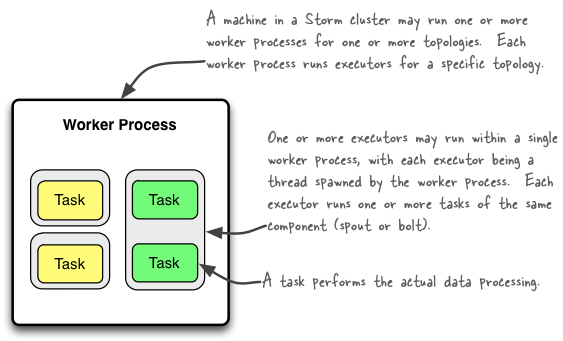
\includegraphics[width=\linewidth]{images/Storm_worker-processes_executors_tasks.png}}
	\caption{The relationships of worker processes, executors
          (threads) and tasks in Storm, adopted from
          \cite{www-noll2012-parallelismofstormtopology} }
	\label{fig:Storm_worker-processes_executors_tasks}
\end{figure}


\subsection{Running Topology}
A running topology as illustrated in
Fig. \ref{fig:Storm_example_of_a_running_topology}.

\begin{figure}[htbp]
	\centering
	\fbox{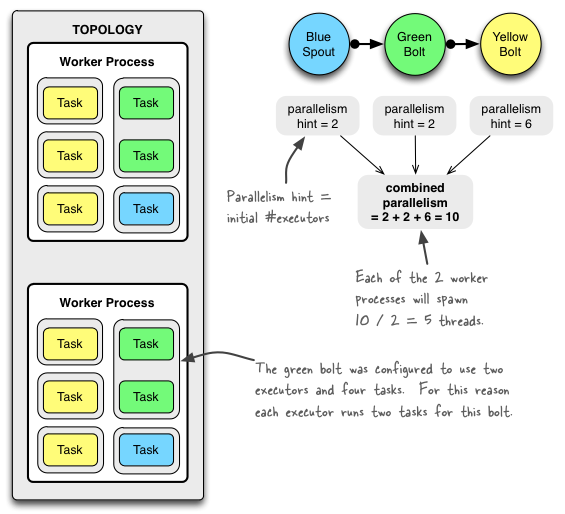
\includegraphics[width=\linewidth]{images/Storm_example_of_a_running_topology.png}}
	\caption{Example of a Running Topology, adopted from
	\cite{www-noll2012-parallelismofstormtopology} }
	\label{fig:Storm_example_of_a_running_topology}
\end{figure}


Each of the above worker process is running on the same or different
node in the distributed cluster. Worker process(executor or task)
communicates with other Worker processes.

Apache Storm is a free and open source distributed realtime
computation system. Storm makes it easy to reliably process unbounded
streams of data, doing for realtime processing what Hadoop did for
batch processing \cite{www-storm}.

As per \cite{article-nabi2014streams}, Users are free to stitch
together a directed graph of execution, with Spouts (data sources) and
Bolts (operators). Architecturally, it consists of a central job and
node management entity dubbed the Nimbus node, and a set of per-node
managers called Supervisors. The Nimbus node is in charge of work
distribution, job orchestration, communication, fault-tolerance, and
state management (for which it relies on ZooKeeper).

The parallelism of a Topology can be controlled at 3 different levels:
number of workers (cluster wide processes), executors (number of
threads per worker), and tasks (number of bolts/spouts executed per
thread)

Communication is handled at different levels in Storm using-
\begin{itemize}
  \renewcommand{\labelitemi}{\scriptsize$\square$}
        \item Intra-worker communication in Storm (inter-thread on the
          same Storm node): using LMAX Disruptor
        \item Inter-worker communication (node-to-node across
          the network): using ZeroMQ or Netty
        \item Inter-topology communication: nothing
built into Storm, you must take care of this yourself with e.g. a
messaging system such as Kafka/RabbitMQ, a database, etc.
\end{itemize}

For inter-worker communication Storm uses ZeroMQ by default in older
versions and can use Netty in Storm versions later than 0.9, as the
network messaging backend.

\section{Performance - Yahoo Engineering Experiment}

Yahoo experimented in 2013 for using a pluggable messaging layer for
Inter-worker communication using Netty \cite{article-storm-netty}. A
simple speed of light test was run to benchmark and measure
performance of messaging layer. This can be done by pushing messages
between different Spouts and Bolts.

\subsection{Setup and Configuration of Cluster}
In the cluster setup 38 nodes, 3 nodes were dedicated to Zookeeper, 1
to Nimbus and the UI, and 34 for Supervisor and Logviewer processes.
Each node had 2 x 2.4GHz Xenon processors each with 4 cores and
Hyperthreading enabled for a total of 16 threads of execution.
\TODO{
  \GE
Check Grammar.   
Don't use capitalization unnecessarily. 
}
\subsection{Netty Behavior with large Topology}
The Netty behavior with Topology of 3 workers running on 3 nodes. In
the below Fig \ref{fig:nettyvzmq-small}, the Y-axis represents number
of messages sent and X-axis represent the size of messages. A 100\%
increase in number of messages is seen with Netty as compared to
zeromq.

\begin{figure}[htbp]
	\centering
	\fbox{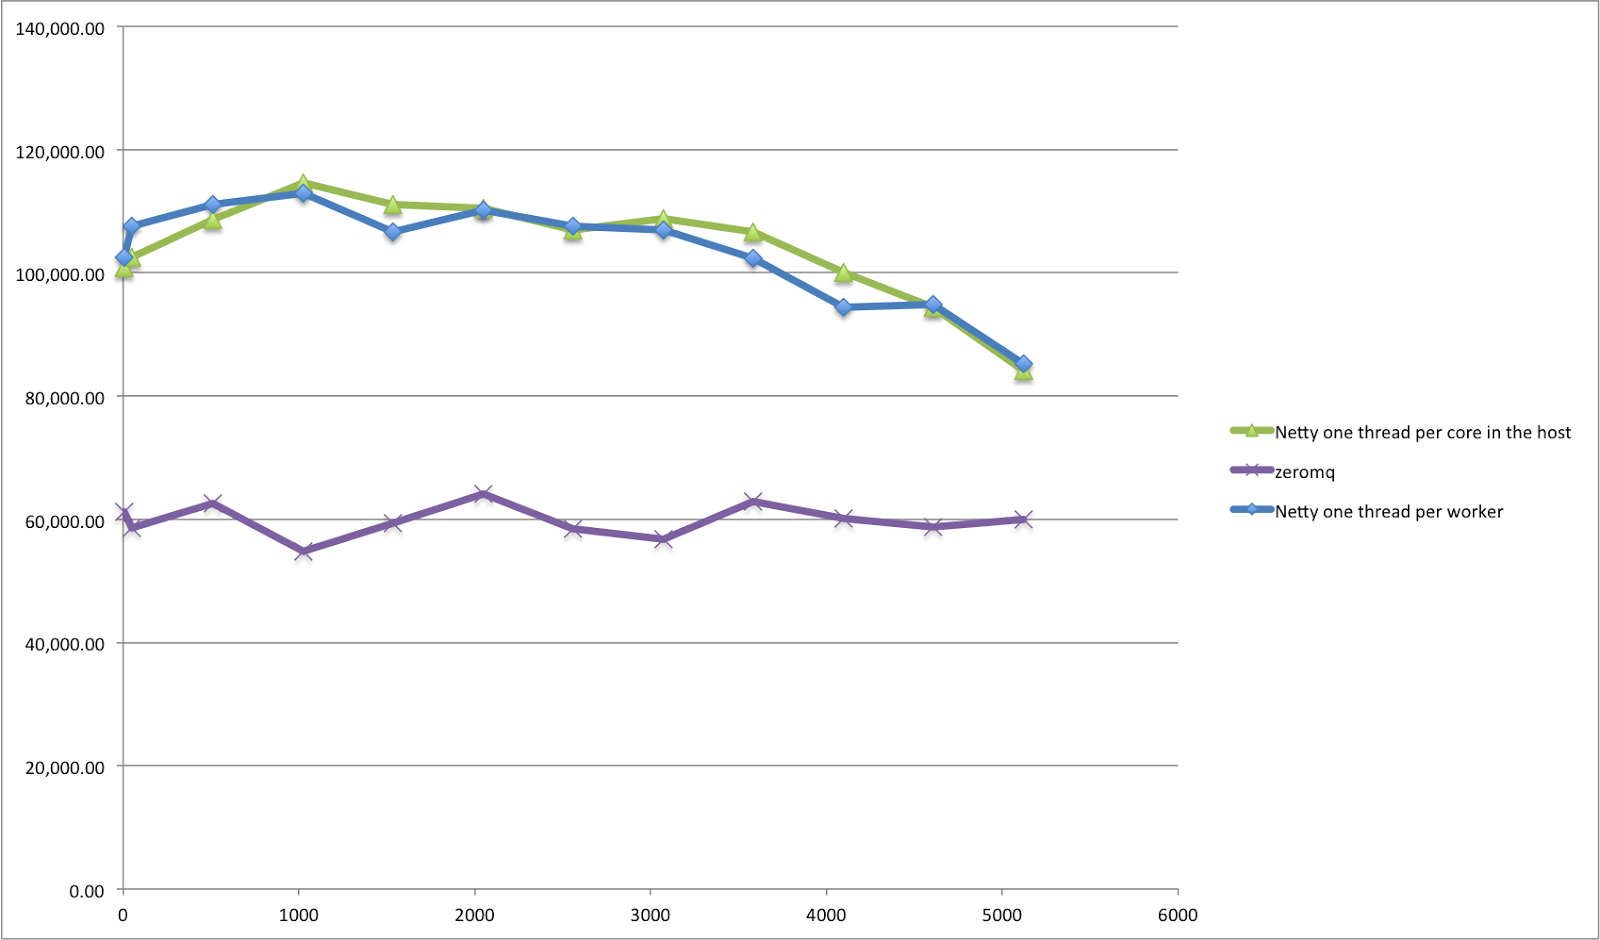
\includegraphics[width=\linewidth]{images/nettyvzmq-small.png}}
	\caption{Small Topology- Netty vs ZeroMQ, adopted from
          \cite{article-storm-netty} }
	\label{fig:nettyvzmq-small}
\end{figure}



\subsection{Netty Behavior with large Topology}
The Netty behavior with Topology of 100 workers, 100 spouts, 500 bolts
spread out in 5 levels of 100 bolts each, and 100 ackers is shown in
Fig \ref{fig:NettyVsZMQFull}.

\begin{figure}[htbp]
	\centering
	\fbox{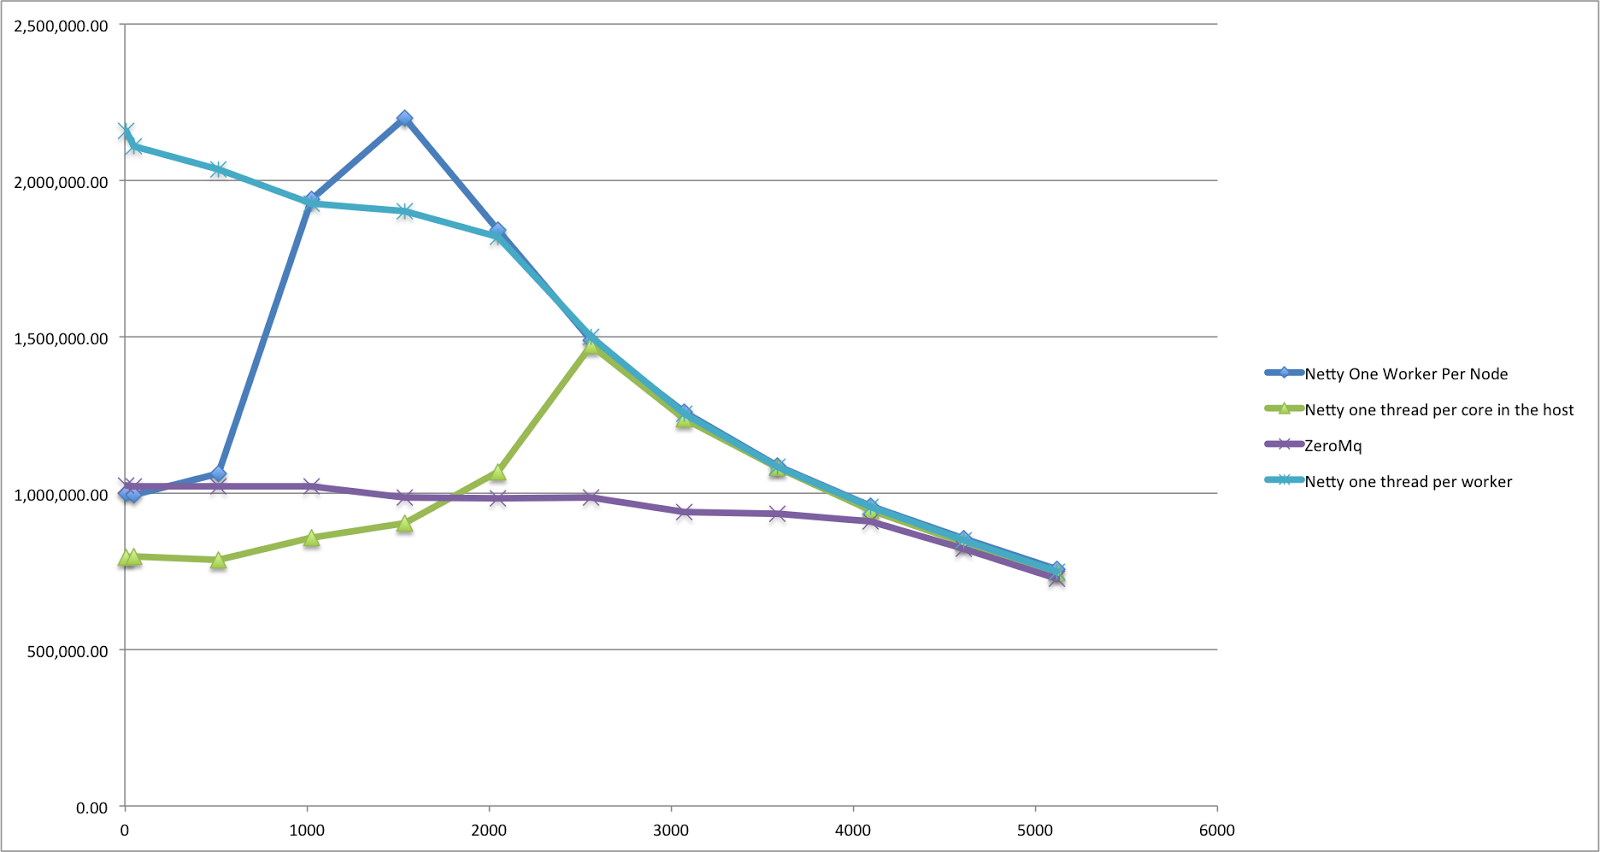
\includegraphics[width=\linewidth]{images/NettyVsZMQFull.png}}
	\caption{Large Topology- Netty vs ZeroMQ, adopted from
          \cite{article-storm-netty}}
	\label{fig:NettyVsZMQFull}
\end{figure}

An increase is seen in number of messages as message size is increased
however above behavior is due to less context switching as the message
size increases. Post a peak at 2.5KB message size, network saturation
occurs and we see a slope down where Netty performance matches ZeroMQ
at 4KB message size.

To resolve and better Netty performance we need to-
\begin{itemize}
	\renewcommand{\labelitemi}{\scriptsize$\square$} 
	\item Reduce number of workers so single worker is running per
          node
        \item Make the number of threads configurable to default 1,
          which matches ZeroMQ default.
\end{itemize}

\section{Performance - IBM Experiment}
Another verification of the numbers stated by Yahoo was done in IBM
Whitepaper "Of streams and storms" \cite{article-nabi2014streams}.

In \cite{article-nabi2014streams},the performance benchmarking is
carried out by processing an Enron email dataset of half a million
emails through data processing pipeline. The processing pipeline used
IBM Infosphere Stream versus Apache Storm.
\TODO{
Full-stop missing. 
}
\subsection{Setup and Configuration of Cluster}
The cluster here consists of 6-nodes, 1 Nimbus node, 1 Zookeeper, 4
Supervisory nodes. Each node with 3GHz dual-core Xeon cluster (HS21),
2 CPUs per node, 8GB RAM, dual 146GB drives, RHEL 6.2 It is mentioned
in the paper that Storm with Netty is around 1.65 times faster (in
terms of throughput) than Storm with ZeroMQ for a multinode setup and
“Restricted Benchmark” which consists of a simple 3-stage pipeline:
source, count, and sink on a 4-node configuration

\subsection{Report of Throughput}
The below table shows the throughput number improvement for Storm with
Netty(Storm 0.8.2) vs Storm with ZeroMQ(Storm 0.9.0.1) in
Fig. \ref{fig:OfStreamsAndStorms}.

\begin{figure}[htbp]
	\centering
	\fbox{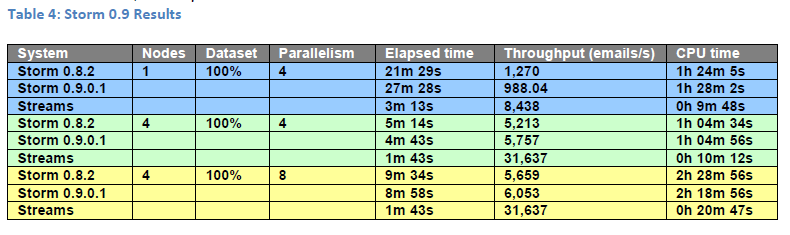
\includegraphics[width=\linewidth]{images/OfStreamsAndStorms.png}}
	\caption{Storm Results 0.9 vs 0.8.2, adopted from
          \cite[p.~27]{article-nabi2014streams}}
	\label{fig:OfStreamsAndStorms}
\end{figure}

\TODO{
  \SE
  *tuning
  Improve conclusion. 
}

\section{Conclusion}
Netty can be used as a pluggable Messaging framework for Distributed
Computation System for Realtime Analytics for performance improvement
however there is restriction of currently using it only for inter
process communication. Netty is a pure Java solution which has a
higher memory footprint of the application in comparison to ZeroMQ
hence tuning is required for JVM heap size.

\bibliography{references}
 

\end{document}
